% Options for packages loaded elsewhere
\PassOptionsToPackage{unicode}{hyperref}
\PassOptionsToPackage{hyphens}{url}
% !TeX program = pdfLaTeX
\documentclass[12pt]{article}
\usepackage{amsmath}
\usepackage{graphicx,psfrag,epsf}
\usepackage{enumerate}
\usepackage[]{natbib}
\usepackage{textcomp}


%\pdfminorversion=4
% NOTE: To produce blinded version, replace "0" with "1" below.
\newcommand{\blind}{0}

% DON'T change margins - should be 1 inch all around.
\addtolength{\oddsidemargin}{-.5in}%
\addtolength{\evensidemargin}{-1in}%
\addtolength{\textwidth}{1in}%
\addtolength{\textheight}{1.7in}%
\addtolength{\topmargin}{-1in}%

%% load any required packages here


% Pandoc syntax highlighting
\usepackage{color}
\usepackage{fancyvrb}
\newcommand{\VerbBar}{|}
\newcommand{\VERB}{\Verb[commandchars=\\\{\}]}
\DefineVerbatimEnvironment{Highlighting}{Verbatim}{commandchars=\\\{\}}
% Add ',fontsize=\small' for more characters per line
\usepackage{framed}
\definecolor{shadecolor}{RGB}{248,248,248}
\newenvironment{Shaded}{\begin{snugshade}}{\end{snugshade}}
\newcommand{\AlertTok}[1]{\textcolor[rgb]{0.94,0.16,0.16}{#1}}
\newcommand{\AnnotationTok}[1]{\textcolor[rgb]{0.56,0.35,0.01}{\textbf{\textit{#1}}}}
\newcommand{\AttributeTok}[1]{\textcolor[rgb]{0.13,0.29,0.53}{#1}}
\newcommand{\BaseNTok}[1]{\textcolor[rgb]{0.00,0.00,0.81}{#1}}
\newcommand{\BuiltInTok}[1]{#1}
\newcommand{\CharTok}[1]{\textcolor[rgb]{0.31,0.60,0.02}{#1}}
\newcommand{\CommentTok}[1]{\textcolor[rgb]{0.56,0.35,0.01}{\textit{#1}}}
\newcommand{\CommentVarTok}[1]{\textcolor[rgb]{0.56,0.35,0.01}{\textbf{\textit{#1}}}}
\newcommand{\ConstantTok}[1]{\textcolor[rgb]{0.56,0.35,0.01}{#1}}
\newcommand{\ControlFlowTok}[1]{\textcolor[rgb]{0.13,0.29,0.53}{\textbf{#1}}}
\newcommand{\DataTypeTok}[1]{\textcolor[rgb]{0.13,0.29,0.53}{#1}}
\newcommand{\DecValTok}[1]{\textcolor[rgb]{0.00,0.00,0.81}{#1}}
\newcommand{\DocumentationTok}[1]{\textcolor[rgb]{0.56,0.35,0.01}{\textbf{\textit{#1}}}}
\newcommand{\ErrorTok}[1]{\textcolor[rgb]{0.64,0.00,0.00}{\textbf{#1}}}
\newcommand{\ExtensionTok}[1]{#1}
\newcommand{\FloatTok}[1]{\textcolor[rgb]{0.00,0.00,0.81}{#1}}
\newcommand{\FunctionTok}[1]{\textcolor[rgb]{0.13,0.29,0.53}{\textbf{#1}}}
\newcommand{\ImportTok}[1]{#1}
\newcommand{\InformationTok}[1]{\textcolor[rgb]{0.56,0.35,0.01}{\textbf{\textit{#1}}}}
\newcommand{\KeywordTok}[1]{\textcolor[rgb]{0.13,0.29,0.53}{\textbf{#1}}}
\newcommand{\NormalTok}[1]{#1}
\newcommand{\OperatorTok}[1]{\textcolor[rgb]{0.81,0.36,0.00}{\textbf{#1}}}
\newcommand{\OtherTok}[1]{\textcolor[rgb]{0.56,0.35,0.01}{#1}}
\newcommand{\PreprocessorTok}[1]{\textcolor[rgb]{0.56,0.35,0.01}{\textit{#1}}}
\newcommand{\RegionMarkerTok}[1]{#1}
\newcommand{\SpecialCharTok}[1]{\textcolor[rgb]{0.81,0.36,0.00}{\textbf{#1}}}
\newcommand{\SpecialStringTok}[1]{\textcolor[rgb]{0.31,0.60,0.02}{#1}}
\newcommand{\StringTok}[1]{\textcolor[rgb]{0.31,0.60,0.02}{#1}}
\newcommand{\VariableTok}[1]{\textcolor[rgb]{0.00,0.00,0.00}{#1}}
\newcommand{\VerbatimStringTok}[1]{\textcolor[rgb]{0.31,0.60,0.02}{#1}}
\newcommand{\WarningTok}[1]{\textcolor[rgb]{0.56,0.35,0.01}{\textbf{\textit{#1}}}}

% tightlist command for lists without linebreak
\providecommand{\tightlist}{%
  \setlength{\itemsep}{0pt}\setlength{\parskip}{0pt}}



\usepackage{booktabs}
\usepackage{longtable}
\usepackage{array}
\usepackage{multirow}
\usepackage{wrapfig}
\usepackage{float}
\usepackage{colortbl}
\usepackage{pdflscape}
\usepackage{tabu}
\usepackage{threeparttable}
\usepackage{threeparttablex}
\usepackage[normalem]{ulem}
\usepackage{makecell}
\usepackage{xcolor}

\IfFileExists{bookmark.sty}{\usepackage{bookmark}}{\usepackage{hyperref}}
\IfFileExists{xurl.sty}{\usepackage{xurl}}{} % add URL line breaks if available
\hypersetup{
  pdftitle={Using Gaussian Mixture Models to Deconstruct Data With Unusual Distributions},
  pdfkeywords={Probability density function; Expectation maximization
algorithm; Multimodality; Pattern recognition; Covariance; k-means
clustering},
  hidelinks,
  pdfcreator={LaTeX via pandoc}}



\begin{document}


\def\spacingset#1{\renewcommand{\baselinestretch}%
{#1}\small\normalsize} \spacingset{1}


%%%%%%%%%%%%%%%%%%%%%%%%%%%%%%%%%%%%%%%%%%%%%%%%%%%%%%%%%%%%%%%%%%%%%%%%%%%%%%

\if0\blind
{
  \title{\bf Using Gaussian Mixture Models to Deconstruct Data With
Unusual Distributions}

  \author{
        Cassandra Jin \thanks{The author gratefully acknowledges
Professor Amy Wagaman for her enriching guidance and patient support in
STAT-495. Professor Wagaman's instruction throughout the course has
allowed for an incredible amount of technical and personal growth, and
this project is has been a wonderful opportunity to apply my skills as
well as to learn more invaluable ones.} \\
    Department of Mathematics and Statistics, Amherst College\\
      }
  \maketitle
} \fi

\if1\blind
{
  \bigskip
  \bigskip
  \bigskip
  \begin{center}
    {\LARGE\bf Using Gaussian Mixture Models to Deconstruct Data With
Unusual Distributions}
  \end{center}
  \medskip
} \fi

\bigskip
\begin{abstract}
This paper explores the fundamental concepts that underpin Gaussian
mixture models (GMM), offering a comprehensive overview of their
mathematical formulation, the Expectation-Maximization (EM) algorithm
employed for parameter estimation, and the principles that govern their
probabilistic nature. The GMM is a generalization of k-means clustering
and is used for decomposing multimodal data into multiple component
distributions, namely Gaussian ones. This paper will thus include an
overview of the Gaussian distribution and go deeper into the utility of
covariance matrices. It will demonstrate how to implement GMM functions
in R and how these apply to real-world applications where GMMs have
demonstrated remarkable efficacy, illustrating their relevance and
versatility across diverse domains.
\end{abstract}

\noindent%
{\it Keywords:} Probability density function; Expectation maximization
algorithm; Multimodality; Pattern recognition; Covariance; k-means
clustering

\vfill

\newpage
\spacingset{1.9} % DON'T change the spacing!

\hypertarget{introduction}{%
\section{Introduction}\label{introduction}}

In the landscape of machine learning, pattern recognition, and data
analysis, the objective and the challenge often lie in capturing
intricate data distributions as effectively as possible. It may be
convenient to assign a single distribution that seems to fit well enough
to a large data set, but it is much more insightful to identify patterns
and clusters within the data. Clustering algorithms such as k-means
clustering provide solutions to finding the patterns within
observations, but such traditional methods still have limitations when
it comes to identifying clusters of different shapes and sizes. For
working with a diverse data set, the Gaussian mixture model (GMM)
employs a combination of multiple Gaussian distributions and, as a
result, excels at capturing the various latent structures within the
data \citep{kumar2022gaussian}.

\begin{figure}
\centering
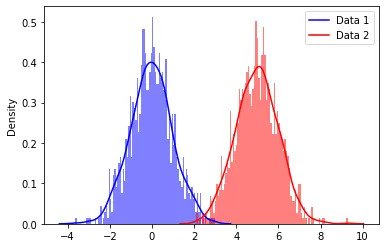
\includegraphics{3.jpg}
\caption{A multimodal distribution, where each peak represents a
different Gaussian distribution or the cluster in the dataset (Ravihara,
2023).}
\end{figure}

We understand k-means clustering to be a method that partitions
observations into \(k\) clusters in which each observation belongs to
the cluster with the nearest mean. Like k-means clustering, the GMM is a
type of machine learning algorithm, but instead, it groups data into
different categories based on any underlying probability distributions.
By identifying and merging multiple Gaussian components, the GMM
achieves a parametric probability density function represented as a
weighted sum of the densities corresponding to each Gaussian component
\citep{reynolds2009gaussian}. The parameters in the method are estimated
from training data using the iterative expectation-maximization (EM)
algorithm, and in maximizing likelihood, GMM allows a representation of
data that goes beyond the limitations of single-distribution models
\citep{bouguila2020mixture}. The method's ability to model a wide array
of distributions (multimodal, non-Gaussian, etc.) has made GMMs
essential in various domains such as computer vision, speech
recognition, anomaly detection, finance, marketing, and more.

This paper aims to guide readers through the fundamental concepts that
underpin GMMs, offering a comprehensive overview of their mathematical
formulation, the Expectation-Maximization (EM) algorithm employed for
parameter estimation, and the principles that govern their probabilistic
nature. Furthermore, we will explore real-world applications where GMMs
have demonstrated remarkable efficacy, illustrating their relevance and
versatility across diverse domains.

\hypertarget{gaussian-mixture-models-gmms}{%
\section{Gaussian Mixture Models
(GMMs)}\label{gaussian-mixture-models-gmms}}

\label{sec:background}

\hypertarget{the-gaussian-distribution}{%
\subsection{The Gaussian Distribution}\label{the-gaussian-distribution}}

The most basic concept in probability theory and in statistics is the
random variable. A random variable can be understood as a mapping from a
random experiment to a variable, and depending on the nature of the
experiment and the design of the mapping, a random variable can take on
discrete values, continuous values, or a mix of discrete and continuous
values. One possible distribution that the resulting values may follow
is the singular Gaussian distribution, which has probability density
function (PDF)

\begin{align} R_X(t, s) &= E[A \cos \omega t \cdot A \cos \omega s] \\ &= A^2 E[\cos \omega t \cos \omega s] \end{align}

\begin{equation}
\label{single}
p(x) = \frac{1}{(2\pi)^{1/2} \sigma} exp(-\frac{1}{2}(\frac{x-\mu}{\sigma})^2) \dot{=} N(x; \mu, \sigma^2),
\end{equation}

or \(x \sim N(\mu, \sigma^2)\), where \(x\) is a continuous random
variable obeying a normal distribution with mean \(\mu\) and variance
\(\sigma^2\).

The Gaussian distribution is commonly used in many engineering and
science disciplines due to its highly desirable computational
properties, but also from its ability to approximate many naturally
occurring real-world distributions, due to the law of large numbers
(Ravihara, 2023).

Expanding this definition to incorporate the weights of component
distributions, \(c_m\), we have that a continuous random variable has a
Gaussian-mixture distribution if its PDF is specified by

\begin{equation}
\label{mix}
p(x) = \sum_{m=1}^M \frac{c_m}{(2\pi)^{1/2} \sigma_m} exp(-\frac{1}{2}(\frac{x-\mu_m}{\sigma_m})^2) = \sum_{m=1}^M c_m N(\mu_m, \sigma_m^2),
\end{equation}

where \(\infty < x < \infty\), \(\sigma_m > 0\), and \(c_m > 0\)
\citep{yu2015gaussian}.

These positive mixture weights must sum to 1: \(\sum_{m=1}^M c_m = 1\),
i.e.~the component distributions combine to describe the full mixture
model.

The most obvious property of Gaussian mixture distribution is its
multimodality (\(M>1\) in Equation \ref{mix}), in contrast to the
unimodal property of the Gaussian distribution where \(M=1\). This makes
it possible for a GMM to adequately describe many types of physical data
exhibiting multimodality, which are poorly suited for a single Gaussian
distribution.

Based on Equation \ref{mix}, the expectation of a random variable \(x\)
with the mixture Gaussian PDF is \(E(x) = \sum_{m=1}^M c_m \mu_m\). But
unlike a singular, unimodal Gaussian distribution, this simple summary
statistic is not very informative unless all the component means,
\(\mu_m\) for \(m = 1, ..., M\), in the Gaussian-mixture distribution
are close to each other.

Instead, we use the multivariate generalization of the mixture Gaussian
distribution, which has joint PDF

\begin{equation}
\label{joint}
p(x) = \sum_{m=1}^M \frac{c_m}{(2\pi)^{D/2} |\Sigma_m|^{1/2}} exp(-\frac{1}{2}(x-\mu_m)^T \Sigma_m^{-1}(x-\mu_m)) = \sum_{m=1}^M c_m N(x; \mu_m, \Sigma_m),
\end{equation}

where \(D\) is random variable \(x\)'s dimensionality, \(\Sigma_m\)
holds the covariance matrices, and \(c_m > 0\) still.

In using the multivariate mixture Gaussian distribution of Equation
\ref{mix}, if \(D\) is large (this depends on the context), then the use
of full (nondiagonal) covariance matrices (\(\Sigma_m\)) would involve a
large number of parameters \citep{bouguila2020mixture}. To reduce the
number of parameters, one can instead use diagonal covariance matrices
for \(\Sigma_m\). Alternatively, when \(M\) is large, one can also
constrain all covariance matrices to be the same. The advantage of using
diagonal covariance matrices is significant simplification of
computations needed for the applications of the Gaussian-mixture
distributions \citep{wan2019novel}.

\hypertarget{parameter-estimation}{%
\subsection{Parameter Estimation}\label{parameter-estimation}}

The Gaussian-mixture distributions discussed above contain a set of
parameters. In the multivariate case of Equation \ref{mix}, the
parameter set consists of \(\Theta = \{c_m, \mu_m, \Sigma_m\}\). The
parameter estimation problem is motivated by wanting to determine the
values of these parameters from data set that we assume to be drawn from
the Gaussian-mixture distribution.

It is common to think of Gaussian mixture modeling and the related
parameter estimation as a missing data problem. We want to ``learn''
appropriate parameters for the distribution, with the connection to the
data points being represented as their membership in the individual
Gaussian distributions.

Here, we focus on the expectation maximization (EM) algorithm as the
maximum likelihood method of choice for parameter estimation of the
Gaussian-mixture distribution. The EM algorithm is the most popular
technique used to estimate the parameters of a mixture given a fixed
number of mixture components, and it can be used to compute the
parameters of any parametric mixture distribution. The EM algorithm
finds the maximum likelihood of a model through two iterative steps: an
expectation or E-step and a maximization or M-step. It alternates
between performing an expectation step and a maximization step to
achieve maximum likelihood until a certain stop condition is satisfied
or a specified number of iterations is completed \citep{wan2019novel}.

The EM algorithm is especially fitting to use for GMM, as we can express
the parameters in their closed forms and iterate through the M-step
\citep{do2008expectation}. Given the current estimate for the
parameters, denoted by just a superscript in the closed forms, the
conditional probability for a given observation \(x^{(t)}\) generated
from a mixture component \(m\) is determined for each data sample point
at \(t=1, ..., N\), where \(N\) is the sample size. The parameters then
update such that the new component weights correspond to the average
conditional probability, and each component mean and covariance is the
component specific weighted average of the mean and covariance of the
entire sample set.

A particular advantage of the EM algorithm is that each successive
iteration will not decrease the likelihood, a property not shared by
many other maximization techniques \citep{reynolds2009gaussian}.
Additionally, the EM algorithm naturally embeds constraints on the
probability vector while avoiding extra computational costs to check and
maintain appropriate values \citep{yu2015gaussian}. On the other hand,
the EM algorithm can be too sensitive to initial values and may falsely
identify local maxima. This problem can be addressed by evaluating at
several initial points in the parameter space, but this may become
computationally costly and undo the advantageous efficiency of the
algorithm.

\hypertarget{summary}{%
\subsection{Summary}\label{summary}}

Overall, there are three key steps to using Gaussian mixture models for
clustering:

\begin{enumerate}
\def\labelenumi{\arabic{enumi}.}
\item
  Determine a covariance matrix that defines how each Gaussian is
  related to one another. The more similar two Gaussian component
  distributions are, the closer their means will be and vice versa if
  they are far away from each other in terms of similarity. A GMM can
  have a covariance matrix that is diagonal or symmetric (non-diagonal).
\item
  Decide the number of Gaussian component distributions, which dictates
  how many clusters are present in the model.
\item
  Select the hyperparameters that define how the data are optimally
  separated using GMMs.
\end{enumerate}

\hypertarget{connections-and-comparisons-to-other-models}{%
\section{Connections and Comparisons to Other
Models}\label{connections-and-comparisons-to-other-models}}

\label{sec:compare}

Compared with traditional k-means clustering algorithm, GMM has two
primary advantages. Firstly, it takes into account covariance, which
determines the shape of the distribution, so it can fit well when the
distribution of the data presents different shapes. Secondly, while
k-means results in hard clustering, GMM is able to perform a more
flexible clustering on data, called soft clustering (``Cluster Using
Gaussian Mixture Model'', 2023). Soft clustering methods assign a score
to each data point in a cluster to represent the association strength of
the data point to the cluster. As opposed to how hard clustering
(k-means) outputs a specific category for each data point, soft
clustering (GMM) is flexible in that it can assign a data point to more
than one cluster and it outputs the probability of each specific
category the data points belong to. Thus, the GMM yields an estimated
uncertainty measure of the degree of association between data points and
specific categories \citep{huang2023gaussian}.

As a trade-off of GMMs being more flexible than k-means, they can be
more difficult to train. K-means is typically faster to converge and
more accurate, so it may be preferred in cases where the runtime is an
important consideration or generally when the data set is large and the
clusters are well-separated. On the other hand, GMMs are more accurate
when the data set is small or the clusters are not well-separated
\citep{kumar2022gaussian}.

We know that the EM algorithm enables effective parameter estimation in
probabilistic models with incomplete data. By implementing this
algorithm, Gaussian mixture models can handle missing data, whereas
K-means cannot. This difference makes GMMs more effective in certain
applications where the data contains considerable noise or is not
well-defined.

\hypertarget{applications-in-literature}{%
\section{Applications in Literature}\label{applications-in-literature}}

\label{sec:examples}

\begin{itemize}
\tightlist
\item
  Understanding the impact of COVID-19 on energy consumption:
  Researchers used the electricity data set of public buildings in
  Scotland and applied Gaussian Mixture Model (GMM) to explore the
  changes in electricity usage patterns throughout the pandemic, so as
  to understand the long-term impact of COVID-19 on energy consumption
  of public buildings \citep{huang2023gaussian}.
\end{itemize}

\begin{figure}
\centering
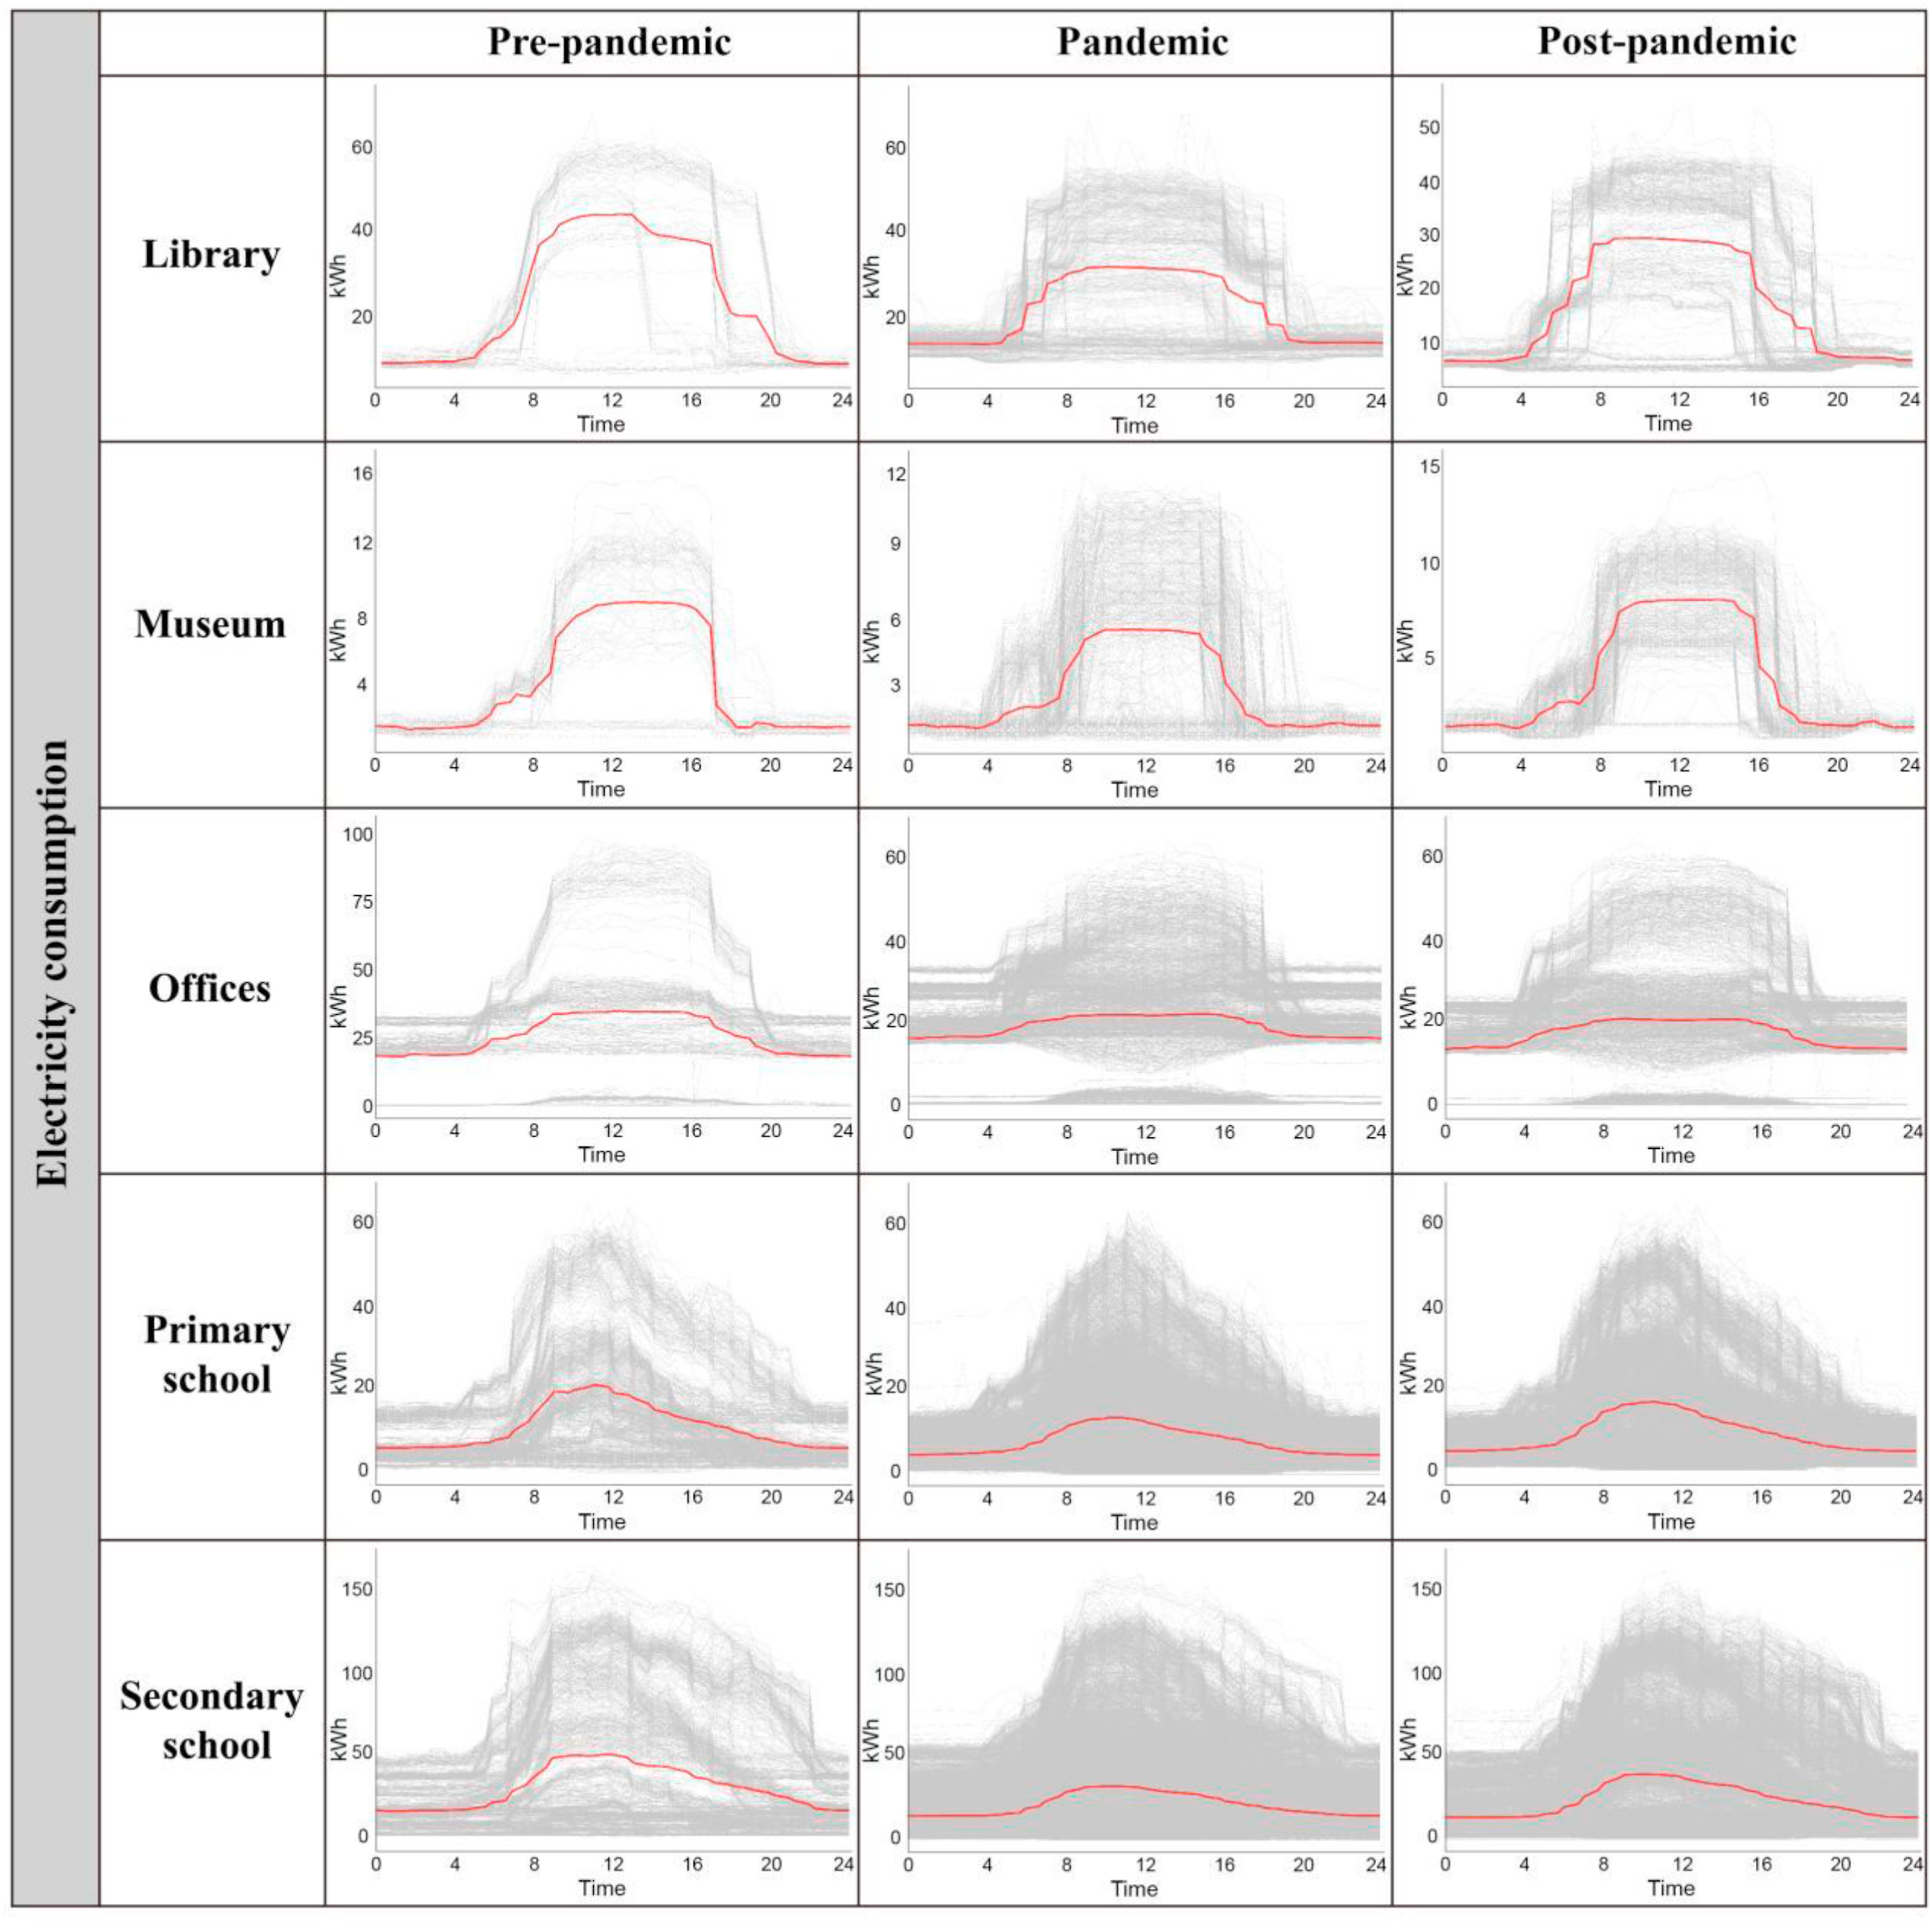
\includegraphics{1.jpg}
\caption{Daily electricity consumption trends of various public
buildings in different periods \citep{huang2023gaussian}.}
\end{figure}

\begin{figure}
\centering
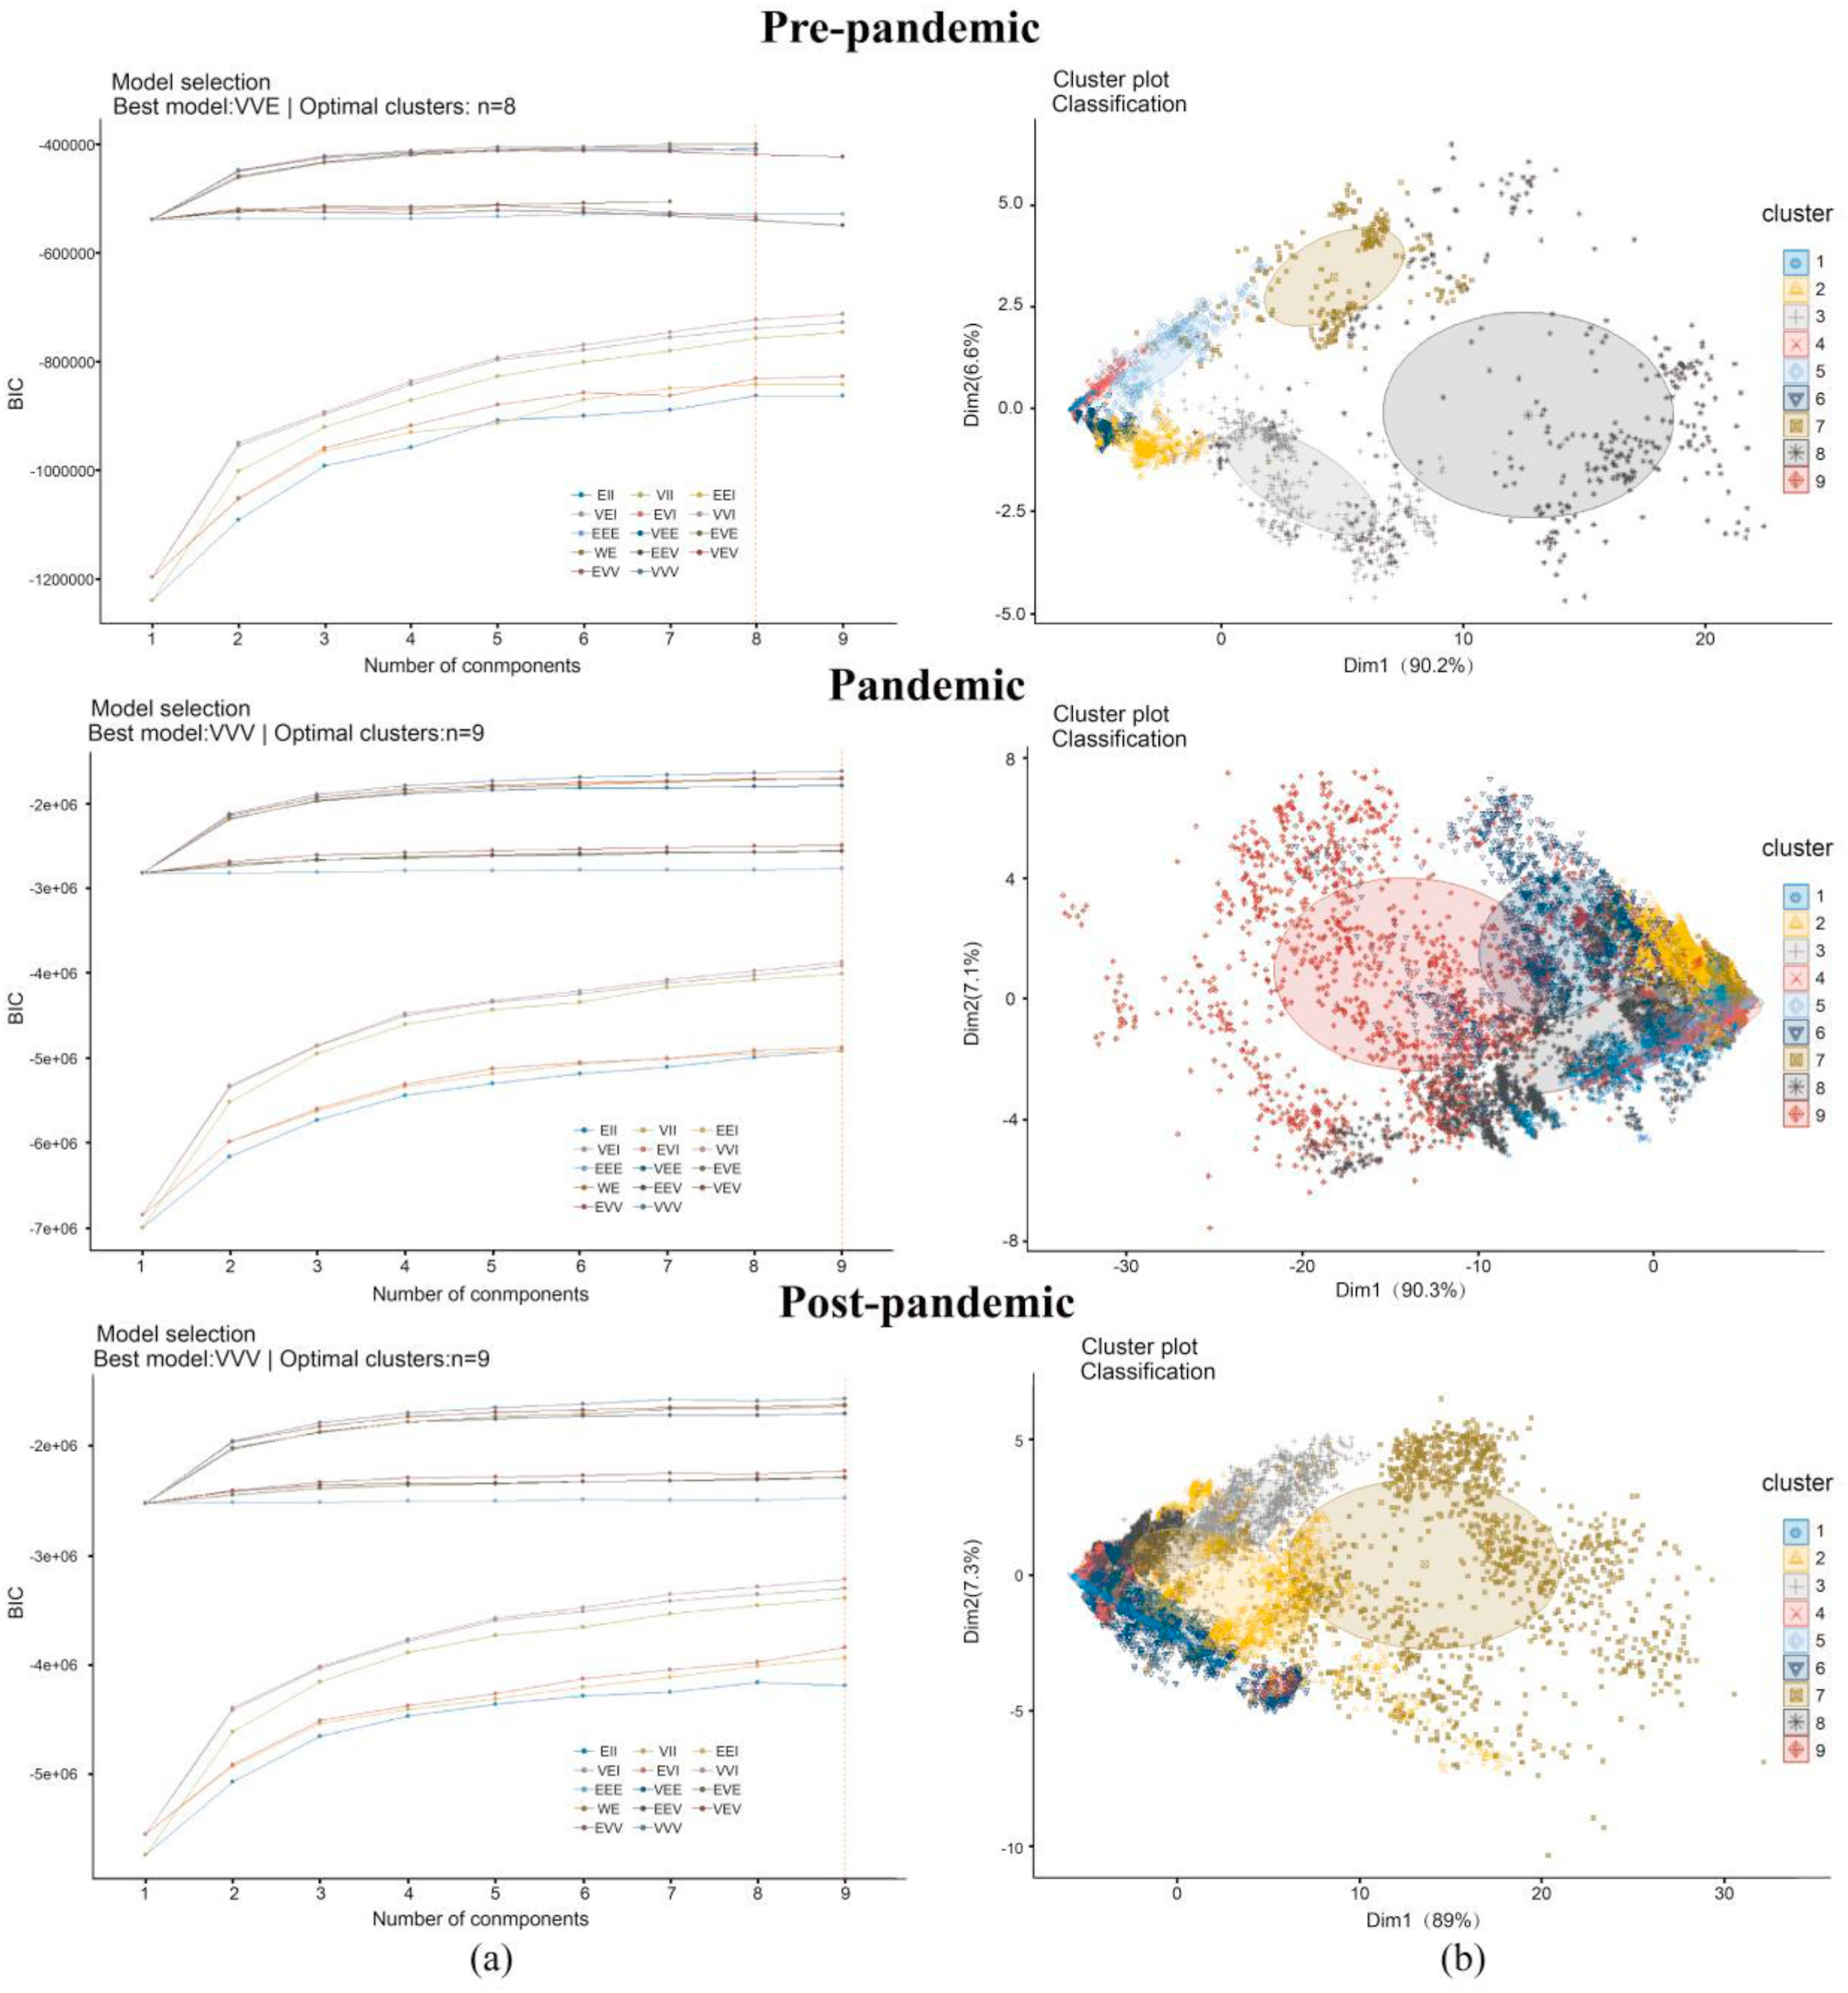
\includegraphics{2.jpg}
\caption{On the right, (b), the visualized Gaussian mixture model for
each condition \citep{huang2023gaussian}.}
\end{figure}

\begin{itemize}
\item
  Finding patterns in medical datasets: Medical researchers use GMMs to
  segment images into multiple categories based on their content or to
  find specific patterns in medical datasets. They can determine
  clusters of patients with similar symptoms, identify disease subtypes,
  and even predict outcomes \citep{riaz2020gaussian}.
\item
  Modeling natural phenomena: GMMs can be used to model natural
  phenomena where it has been found that noise follows Gaussian
  distributions. This model of probabilistic modeling relies on the
  assumption that there exists some underlying continuum of unobserved
  entities or attributes, and that each member is associated with
  measurements taken at equidistant points in multiple observation
  sessions \citep{xi2023deep}.
\item
  Customer behavior analysis: GMMs can be used for performing customer
  behavior analysis in marketing to make predictions about future
  purchases based on historical data \citep{melzi2017dedicated}.
\item
  Stock price prediction: In finance, GMMs can be applied to a stock's
  price time series. They can detect changepoints in time series data
  and help find turning points of stock prices or other market movements
  that are otherwise difficult to spot due to volatility and noise
  \citep{gopinathan2023stock}.
\item
  Gene expression data analysis: GMMs can be used to detect
  differentially expressed genes between two conditions and to identify
  which genes might contribute toward a certain phenotype or disease
  state \citep{mcnicholas2010model}.
\end{itemize}

\hypertarget{implementation-in-r}{%
\section{Implementation in R}\label{implementation-in-r}}

The function \texttt{rGMM} simulates observations from a GMM. The number
of observations is specified by \(n\), and the dimension of each
observation by \(d\), as seen in Equation \ref{joint}. The number of
clusters is set using \(k\), which defaults to 1. We introduce the
parameter of missingness, which is the proportion of elements in the
\(n \times d\) data matrix that are missing and which defaults to zero
\citep{McCaw2019.12.20.884551}. The cluster means and covariances
(\texttt{covs}) are provided as numeric prototype vectors, or lists of
such vectors. In settings where \texttt{miss} \(> 0\) (it is possible
for all elements of an observation to be missing), these vectors are
used as the mean and covariance of all clusters. By default, however,
the zero vector and the identity matrix are adopted for the mean and
covariance, respectively. We will simulate a few cases of data to
demonstrate the functionality of the \texttt{rGMM} function.

\hypertarget{single-component-without-missingness}{%
\subsection{Single Component Without
Missingness}\label{single-component-without-missingness}}

For \(n\) observations on \(d\) dimensional data, we can introduce a
fraction of missing values \(m\) completely at random by setting
elements of the data set to NA.

Here, \(n = 1000\) observations are simulated from a single \(k = 1\)
bivariate normal distribution \(d = 2\) without missingness (miss = 0,
by default). The mean is \(\mu = (2, 2)\), and the covariance is an
exchangeable correlation structure with off-diagonal \(\rho = 0.5\).

\begin{Shaded}
\begin{Highlighting}[]
\FunctionTok{set.seed}\NormalTok{(}\DecValTok{495}\NormalTok{)}
\NormalTok{sigma }\OtherTok{\textless{}{-}} \FunctionTok{matrix}\NormalTok{(}\FunctionTok{c}\NormalTok{(}\DecValTok{1}\NormalTok{, }\FloatTok{0.5}\NormalTok{, }\FloatTok{0.5}\NormalTok{, }\DecValTok{1}\NormalTok{), }\AttributeTok{nrow =} \DecValTok{2}\NormalTok{)}
\NormalTok{data }\OtherTok{=} \FunctionTok{rGMM}\NormalTok{(}\AttributeTok{n =} \FloatTok{1e3}\NormalTok{, }\AttributeTok{d =} \DecValTok{2}\NormalTok{, }\AttributeTok{k =} \DecValTok{1}\NormalTok{, }\AttributeTok{means =} \FunctionTok{c}\NormalTok{(}\DecValTok{2}\NormalTok{, }\DecValTok{2}\NormalTok{), }\AttributeTok{covs =}\NormalTok{ sigma)}
\NormalTok{fit }\OtherTok{\textless{}{-}} \FunctionTok{FitGMM}\NormalTok{(data, }\AttributeTok{k =} \DecValTok{1}\NormalTok{)}
\FunctionTok{show}\NormalTok{(fit)}
\end{Highlighting}
\end{Shaded}

\begin{verbatim}
## Multivariate Normal Model. 
## 
## Estimated mean:
##   y1   y2 
## 2.01 2.00 
## 
## Estimated covariance:
##       y1    y2
## y1 0.963 0.475
## y2 0.475 1.020
## 
## Final Objective:
## [1] -1720
\end{verbatim}

The \texttt{Estimated\ covariance} table contains values obtained
through fitting a GMM with the \texttt{rGMM} function on generated data,
and we see that they are close to the target covariance values of \{1,
0.5, 0.5, 1\}.

\hypertarget{single-component-with-missingness}{%
\subsection{Single Component With
Missingness}\label{single-component-with-missingness}}

\(n = 1000\) observations are simulated from a single \(k = 1\)
trivariate normal distribution \(d = 3\) with 20\% missingness (miss =
0.2). The mean defaults to the zero vector, and the covariance to the
identity matrix.

\begin{Shaded}
\begin{Highlighting}[]
\FunctionTok{set.seed}\NormalTok{(}\DecValTok{495}\NormalTok{)}
\NormalTok{sigma }\OtherTok{\textless{}{-}} \FunctionTok{matrix}\NormalTok{(}\FunctionTok{c}\NormalTok{(}\DecValTok{1}\NormalTok{, }\FloatTok{0.5}\NormalTok{, }\FloatTok{0.5}\NormalTok{, }\DecValTok{1}\NormalTok{), }\AttributeTok{nrow =} \DecValTok{2}\NormalTok{)}
\NormalTok{data }\OtherTok{=} \FunctionTok{rGMM}\NormalTok{(}\AttributeTok{n =} \FloatTok{1e3}\NormalTok{, }\AttributeTok{d =} \DecValTok{3}\NormalTok{, }\AttributeTok{k =} \DecValTok{1}\NormalTok{, }\AttributeTok{miss =} \FloatTok{0.2}\NormalTok{)}
\NormalTok{fit }\OtherTok{\textless{}{-}} \FunctionTok{FitGMM}\NormalTok{(data, }\AttributeTok{k =} \DecValTok{1}\NormalTok{)}
\end{Highlighting}
\end{Shaded}

\begin{verbatim}
## Objective increment:  2.76 
## Objective increment:  0.135 
## Objective increment:  0.00904 
## Objective increment:  0.000855 
## Objective increment:  0.000101 
## Objective increment:  1.33e-05 
## Objective increment:  1.82e-06 
## Objective increment:  2.55e-07 
## 7 update(s) performed before reaching tolerance limit.
\end{verbatim}

\begin{Shaded}
\begin{Highlighting}[]
\FunctionTok{show}\NormalTok{(fit)}
\end{Highlighting}
\end{Shaded}

\begin{verbatim}
## Multivariate Normal Model. 
## 
## Estimated mean:
##      y1      y2      y3 
## 0.01740 0.02460 0.00185 
## 
## Estimated covariance:
##         y1      y2     y3
## y1  0.9700 -0.0303 0.0227
## y2 -0.0303  1.0400 0.0363
## y3  0.0227  0.0363 1.0700
## 
## Final Objective:
## [1] -3040
\end{verbatim}

Again, we see that the values of the \texttt{Estimated\ mean} vector are
near-zero and those of the \texttt{Estimated\ covariance} matrix closely
follow the identity matrix, as expected in this case.

\hypertarget{cluster-number-selection}{%
\subsection{Cluster Number Selection}\label{cluster-number-selection}}

The function \texttt{ClustQual} provides several metrics for internally
assessing the quality of cluster assignments from a fitted GMM (Arquez,
2020). The output is a list containing the following metrics:

\begin{itemize}
\item
  BIC (Bayesian information criterion): a penalized version of the
  negative log likelihood. A lower value indicates better clustering
  quality.
\item
  CHI (Calinski-Harabaz index): a ratio of the between-cluster to
  within-cluster variation. A higher value indicates better clustering
  quality.
\item
  DBI (Davies-Bouldin index): an average of similarities across
  clusters. A lower value indicates better clustering quality.
\item
  SIL: average silhouette width, a measure of how well an observation
  matches its assigned cluster. A higher value indicates better
  clustering quality.
\end{itemize}

\begin{Shaded}
\begin{Highlighting}[]
\FunctionTok{set.seed}\NormalTok{(}\DecValTok{495}\NormalTok{)}
\NormalTok{mu }\OtherTok{\textless{}{-}} \FunctionTok{list}\NormalTok{(}
  \FunctionTok{c}\NormalTok{(}\DecValTok{2}\NormalTok{, }\DecValTok{2}\NormalTok{),}
  \FunctionTok{c}\NormalTok{(}\DecValTok{2}\NormalTok{, }\SpecialCharTok{{-}}\DecValTok{2}\NormalTok{),}
  \FunctionTok{c}\NormalTok{(}\SpecialCharTok{{-}}\DecValTok{2}\NormalTok{, }\DecValTok{2}\NormalTok{),}
  \FunctionTok{c}\NormalTok{(}\SpecialCharTok{{-}}\DecValTok{2}\NormalTok{, }\SpecialCharTok{{-}}\DecValTok{2}\NormalTok{)}
\NormalTok{)}
\NormalTok{sigma }\OtherTok{\textless{}{-}} \FloatTok{0.5} \SpecialCharTok{*} \FunctionTok{diag}\NormalTok{(}\DecValTok{2}\NormalTok{)}
\NormalTok{data }\OtherTok{=} \FunctionTok{rGMM}\NormalTok{(}\AttributeTok{n =} \DecValTok{100}\NormalTok{, }\AttributeTok{d =} \DecValTok{2}\NormalTok{, }\AttributeTok{k =} \DecValTok{4}\NormalTok{, }\AttributeTok{means =}\NormalTok{ mu, }\AttributeTok{covs =}\NormalTok{ sigma)}
\NormalTok{fit }\OtherTok{\textless{}{-}} \FunctionTok{FitGMM}\NormalTok{(data, }\AttributeTok{k =} \DecValTok{4}\NormalTok{, }\AttributeTok{maxit =} \DecValTok{100}\NormalTok{, }\AttributeTok{eps =} \FloatTok{1e{-}8}\NormalTok{, }\AttributeTok{report =}\NormalTok{ F)}

\CommentTok{\# Quality metrics}
\NormalTok{clust\_qual }\OtherTok{=} \FunctionTok{ClustQual}\NormalTok{(fit)}
\FunctionTok{cat}\NormalTok{(}\StringTok{"BIC:}\SpecialCharTok{\textbackslash{}n}\StringTok{"}\NormalTok{)}
\end{Highlighting}
\end{Shaded}

\begin{verbatim}
## BIC:
\end{verbatim}

\begin{Shaded}
\begin{Highlighting}[]
\NormalTok{clust\_qual}\SpecialCharTok{$}\NormalTok{BIC}
\end{Highlighting}
\end{Shaded}

\begin{verbatim}
## [1] 221.9521
\end{verbatim}

\begin{Shaded}
\begin{Highlighting}[]
\FunctionTok{cat}\NormalTok{(}\StringTok{"}\SpecialCharTok{\textbackslash{}n}\StringTok{CHI:}\SpecialCharTok{\textbackslash{}n}\StringTok{"}\NormalTok{)}
\end{Highlighting}
\end{Shaded}

\begin{verbatim}
## 
## CHI:
\end{verbatim}

\begin{Shaded}
\begin{Highlighting}[]
\NormalTok{clust\_qual}\SpecialCharTok{$}\NormalTok{CHI}
\end{Highlighting}
\end{Shaded}

\begin{verbatim}
## [1] 10.17547
\end{verbatim}

\begin{Shaded}
\begin{Highlighting}[]
\FunctionTok{cat}\NormalTok{(}\StringTok{"}\SpecialCharTok{\textbackslash{}n}\StringTok{DBI:}\SpecialCharTok{\textbackslash{}n}\StringTok{"}\NormalTok{)}
\end{Highlighting}
\end{Shaded}

\begin{verbatim}
## 
## DBI:
\end{verbatim}

\begin{Shaded}
\begin{Highlighting}[]
\NormalTok{clust\_qual}\SpecialCharTok{$}\NormalTok{DBI}
\end{Highlighting}
\end{Shaded}

\begin{verbatim}
## [1] 0.470887
\end{verbatim}

\begin{Shaded}
\begin{Highlighting}[]
\FunctionTok{cat}\NormalTok{(}\StringTok{"}\SpecialCharTok{\textbackslash{}n}\StringTok{SIL:}\SpecialCharTok{\textbackslash{}n}\StringTok{"}\NormalTok{)}
\end{Highlighting}
\end{Shaded}

\begin{verbatim}
## 
## SIL:
\end{verbatim}

\begin{Shaded}
\begin{Highlighting}[]
\NormalTok{clust\_qual}\SpecialCharTok{$}\NormalTok{SIL}
\end{Highlighting}
\end{Shaded}

\begin{verbatim}
## [1] 0.6393902
\end{verbatim}

The biggest question in applying the GMM lies in the unknown number of
clusters \(k\). Using the inputs of the data matrix, the minimum number
of clusters to assess \texttt{k0}, the maximum number of clusters to
assess \texttt{k1}, and the number of bootstrap replicates at each
cluster number boot, the function \texttt{ChooseK} provides guidance on
the number of clusters likely present in the data
\citep{McCaw2019.12.20.884551}. For each cluster number \(k\) from
\texttt{k0} to \texttt{k1}, boot bootstrapped data sets are generated. A
GMM with \(k\) components is fit, and the quality metrics from above are
calculated. The bootstrap replicates are summarized by their mean and
standard error (SE). Thus, for each quality metric, we obtain the
cluster number \texttt{k\_opt} that provided the optimal quality and the
smallest cluster number whose quality was within 1 SE of the optimum
\texttt{k\_1se}.

\begin{Shaded}
\begin{Highlighting}[]
\NormalTok{choose\_k }\OtherTok{\textless{}{-}} \FunctionTok{ChooseK}\NormalTok{(data, }\AttributeTok{k0 =} \DecValTok{2}\NormalTok{, }\AttributeTok{k1 =} \DecValTok{6}\NormalTok{, }\AttributeTok{boot =} \DecValTok{10}\NormalTok{)}
\end{Highlighting}
\end{Shaded}

\begin{verbatim}
## Cluster size 2 complete. 11 fit(s) succeeded.
## Cluster size 3 complete. 11 fit(s) succeeded.
## Cluster size 4 complete. 11 fit(s) succeeded.
## Cluster size 5 complete. 11 fit(s) succeeded.
## Cluster size 6 complete. 10 fit(s) succeeded.
\end{verbatim}

\begin{Shaded}
\begin{Highlighting}[]
\FunctionTok{cat}\NormalTok{(}\StringTok{"}\SpecialCharTok{\textbackslash{}n}\StringTok{Cluster number choices:}\SpecialCharTok{\textbackslash{}n}\StringTok{"}\NormalTok{)}
\end{Highlighting}
\end{Shaded}

\begin{verbatim}
## 
## Cluster number choices:
\end{verbatim}

\begin{Shaded}
\begin{Highlighting}[]
\NormalTok{choose\_k}\SpecialCharTok{$}\NormalTok{Choices}
\end{Highlighting}
\end{Shaded}

\begin{verbatim}
##   Metric k_opt  Metric_opt k_1se  Metric_1se
## 1    BIC     6 151.3227726     5 157.3881681
## 2    CHI     6  15.7701771     6  15.7701771
## 3    DBI     4   0.4754451     4   0.4754451
## 4    SIL     4   0.6443205     4   0.6443205
\end{verbatim}

\begin{Shaded}
\begin{Highlighting}[]
\FunctionTok{cat}\NormalTok{(}\StringTok{"}\SpecialCharTok{\textbackslash{}n}\StringTok{All results:}\SpecialCharTok{\textbackslash{}n}\StringTok{"}\NormalTok{)}
\end{Highlighting}
\end{Shaded}

\begin{verbatim}
## 
## All results:
\end{verbatim}

\begin{Shaded}
\begin{Highlighting}[]
\FunctionTok{head}\NormalTok{(choose\_k}\SpecialCharTok{$}\NormalTok{Results)}
\end{Highlighting}
\end{Shaded}

\begin{verbatim}
##   Clusters Fits Metric        Mean          SE
## 1        2   11    BIC 331.1585430  7.83821234
## 2        2   11    CHI   1.9099133  0.18458241
## 3        2   11    DBI   0.9500322  0.05248028
## 4        2   11    SIL   0.4765720  0.01810555
## 5        3   11    BIC 273.7737692 16.45488885
## 6        3   11    CHI   3.9120636  0.26041417
\end{verbatim}

\hypertarget{application-to-data}{%
\section{Application to Data}\label{application-to-data}}

\begin{Shaded}
\begin{Highlighting}[]
\FunctionTok{data}\NormalTok{(galaxies)}
\end{Highlighting}
\end{Shaded}

\begin{Shaded}
\begin{Highlighting}[]
\CommentTok{\# Multivariate Normal PDF Function Given a matrix x, mu (mean), and}
\CommentTok{\# sigma (covariance), we can calculate the probability density for each}
\CommentTok{\# row using the apply function. The function returns a column vector of}
\CommentTok{\# probabilities.}

\NormalTok{max\_iter }\OtherTok{\textless{}{-}} \DecValTok{100}
\NormalTok{bic\_values }\OtherTok{\textless{}{-}} \FunctionTok{numeric}\NormalTok{(max\_iter)}

\NormalTok{mvpdf }\OtherTok{\textless{}{-}} \ControlFlowTok{function}\NormalTok{(x, mu, sigma) \{}
    \ControlFlowTok{if}\NormalTok{ (}\FunctionTok{det}\NormalTok{(sigma) }\SpecialCharTok{==} \DecValTok{0}\NormalTok{) \{}
        \FunctionTok{warning}\NormalTok{(}\StringTok{"Determinant is equal to 0."}\NormalTok{)}
\NormalTok{    \}}
    \FunctionTok{apply}\NormalTok{(x, }\DecValTok{1}\NormalTok{, }\ControlFlowTok{function}\NormalTok{(x) }\FunctionTok{exp}\NormalTok{(}\SpecialCharTok{{-}}\NormalTok{(}\DecValTok{1}\SpecialCharTok{/}\DecValTok{2}\NormalTok{) }\SpecialCharTok{*}\NormalTok{ (}\FunctionTok{t}\NormalTok{(x) }\SpecialCharTok{{-}}\NormalTok{ mu) }\SpecialCharTok{\%*\%}\NormalTok{ MASS}\SpecialCharTok{::}\FunctionTok{ginv}\NormalTok{(sigma) }\SpecialCharTok{\%*\%} 
        \FunctionTok{t}\NormalTok{(}\FunctionTok{t}\NormalTok{(x) }\SpecialCharTok{{-}}\NormalTok{ mu))}\SpecialCharTok{/}\FunctionTok{sqrt}\NormalTok{(}\FunctionTok{det}\NormalTok{(}\DecValTok{2} \SpecialCharTok{*}\NormalTok{ pi }\SpecialCharTok{*}\NormalTok{ sigma)))}
\NormalTok{\}}

\CommentTok{\# Plot dataset}
\FunctionTok{plot}\NormalTok{(iris[, }\DecValTok{1}\SpecialCharTok{:}\DecValTok{4}\NormalTok{], }\AttributeTok{col =}\NormalTok{ iris}\SpecialCharTok{$}\NormalTok{Species, }\AttributeTok{pch =} \DecValTok{18}\NormalTok{, }\AttributeTok{main =} \StringTok{"Fisher\textquotesingle{}s Iris Dataset"}\NormalTok{)}
\end{Highlighting}
\end{Shaded}

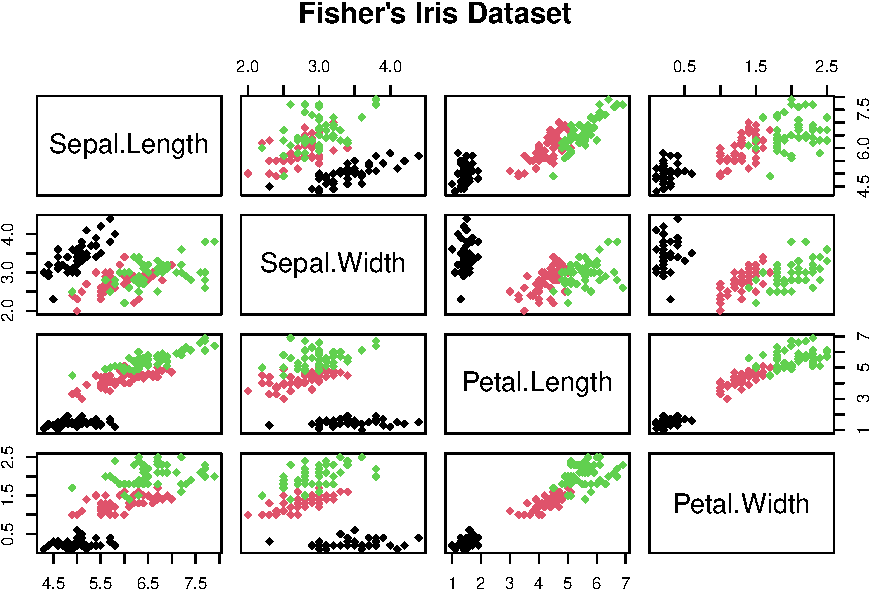
\includegraphics{exposition_files/figure-latex/unnamed-chunk-6-1.pdf}

\begin{Shaded}
\begin{Highlighting}[]
\CommentTok{\# Mclust comes with a method of hierarchical clustering. We\textquotesingle{}ll}
\CommentTok{\# initialize 3 different classes.}
\NormalTok{initialk }\OtherTok{\textless{}{-}} \FunctionTok{hc}\NormalTok{(}\AttributeTok{data =}\NormalTok{ iris, }\AttributeTok{modelName =} \StringTok{"EII"}\NormalTok{)}
\NormalTok{initialk }\OtherTok{\textless{}{-}} \FunctionTok{hclass}\NormalTok{(initialk, }\DecValTok{3}\NormalTok{)}
\CommentTok{\# First split by class and calculate column{-}means for each class.}
\NormalTok{mu }\OtherTok{\textless{}{-}} \FunctionTok{split}\NormalTok{(iris[, }\DecValTok{1}\SpecialCharTok{:}\DecValTok{4}\NormalTok{], initialk)}
\NormalTok{mu }\OtherTok{\textless{}{-}} \FunctionTok{t}\NormalTok{(}\FunctionTok{sapply}\NormalTok{(mu, colMeans))}
\CommentTok{\# Covariance Matrix for each initial class.}
\NormalTok{cov }\OtherTok{\textless{}{-}} \FunctionTok{list}\NormalTok{(}\FunctionTok{diag}\NormalTok{(}\DecValTok{4}\NormalTok{), }\FunctionTok{diag}\NormalTok{(}\DecValTok{4}\NormalTok{), }\FunctionTok{diag}\NormalTok{(}\DecValTok{4}\NormalTok{))}
\CommentTok{\# Mixing Components}
\NormalTok{a }\OtherTok{\textless{}{-}} \FunctionTok{runif}\NormalTok{(}\DecValTok{3}\NormalTok{)}
\NormalTok{a }\OtherTok{\textless{}{-}}\NormalTok{ a}\SpecialCharTok{/}\FunctionTok{sum}\NormalTok{(a)}

\ControlFlowTok{for}\NormalTok{ (iter }\ControlFlowTok{in} \DecValTok{1}\SpecialCharTok{:}\NormalTok{max\_iter) \{}
  
\CommentTok{\# Calculate PDF with class means and covariances.}
\NormalTok{z }\OtherTok{\textless{}{-}} \FunctionTok{cbind}\NormalTok{(}\FunctionTok{mvpdf}\NormalTok{(}\AttributeTok{x =}\NormalTok{ iris[, }\DecValTok{1}\SpecialCharTok{:}\DecValTok{4}\NormalTok{], }\AttributeTok{mu =}\NormalTok{ mu[}\DecValTok{1}\NormalTok{, ], }\AttributeTok{sigma =}\NormalTok{ cov[[}\DecValTok{1}\NormalTok{]]), }\FunctionTok{mvpdf}\NormalTok{(}\AttributeTok{x =}\NormalTok{ iris[, }
    \DecValTok{1}\SpecialCharTok{:}\DecValTok{4}\NormalTok{], }\AttributeTok{mu =}\NormalTok{ mu[}\DecValTok{2}\NormalTok{, ], }\AttributeTok{sigma =}\NormalTok{ cov[[}\DecValTok{2}\NormalTok{]]), }\FunctionTok{mvpdf}\NormalTok{(}\AttributeTok{x =}\NormalTok{ iris[, }\DecValTok{1}\SpecialCharTok{:}\DecValTok{4}\NormalTok{], }\AttributeTok{mu =}\NormalTok{ mu[}\DecValTok{3}\NormalTok{, }
\NormalTok{    ], }\AttributeTok{sigma =}\NormalTok{ cov[[}\DecValTok{3}\NormalTok{]]))}

\CommentTok{\# Expectation Step for each class.}
\NormalTok{r }\OtherTok{\textless{}{-}} \FunctionTok{cbind}\NormalTok{((a[}\DecValTok{1}\NormalTok{] }\SpecialCharTok{*}\NormalTok{ z[, }\DecValTok{1}\NormalTok{])}\SpecialCharTok{/}\FunctionTok{rowSums}\NormalTok{(}\FunctionTok{t}\NormalTok{((}\FunctionTok{t}\NormalTok{(z) }\SpecialCharTok{*}\NormalTok{ a))), (a[}\DecValTok{2}\NormalTok{] }\SpecialCharTok{*}\NormalTok{ z[, }\DecValTok{2}\NormalTok{])}\SpecialCharTok{/}\FunctionTok{rowSums}\NormalTok{(}\FunctionTok{t}\NormalTok{((}\FunctionTok{t}\NormalTok{(z) }\SpecialCharTok{*} 
\NormalTok{    a))), (a[}\DecValTok{3}\NormalTok{] }\SpecialCharTok{*}\NormalTok{ z[, }\DecValTok{3}\NormalTok{])}\SpecialCharTok{/}\FunctionTok{rowSums}\NormalTok{(}\FunctionTok{t}\NormalTok{((}\FunctionTok{t}\NormalTok{(z) }\SpecialCharTok{*}\NormalTok{ a))))}

\CommentTok{\# Choose the highest rowwise probability}
\NormalTok{eK }\OtherTok{\textless{}{-}} \FunctionTok{factor}\NormalTok{(}\FunctionTok{apply}\NormalTok{(r, }\DecValTok{1}\NormalTok{, which.max))}

\CommentTok{\# Total Responsibility}
\NormalTok{mc }\OtherTok{\textless{}{-}} \FunctionTok{colSums}\NormalTok{(r)}

\CommentTok{\# Update Mixing Components.}
\NormalTok{a }\OtherTok{\textless{}{-}}\NormalTok{ mc}\SpecialCharTok{/}\FunctionTok{NROW}\NormalTok{(iris)}

\CommentTok{\# Update our Means}
\NormalTok{mu }\OtherTok{\textless{}{-}} \FunctionTok{rbind}\NormalTok{(}\FunctionTok{colSums}\NormalTok{(iris[, }\DecValTok{1}\SpecialCharTok{:}\DecValTok{4}\NormalTok{] }\SpecialCharTok{*}\NormalTok{ r[, }\DecValTok{1}\NormalTok{]) }\SpecialCharTok{*} \DecValTok{1}\SpecialCharTok{/}\NormalTok{mc[}\DecValTok{1}\NormalTok{], }\FunctionTok{colSums}\NormalTok{(iris[, }\DecValTok{1}\SpecialCharTok{:}\DecValTok{4}\NormalTok{] }\SpecialCharTok{*} 
\NormalTok{    r[, }\DecValTok{2}\NormalTok{]) }\SpecialCharTok{*} \DecValTok{1}\SpecialCharTok{/}\NormalTok{mc[}\DecValTok{2}\NormalTok{], }\FunctionTok{colSums}\NormalTok{(iris[, }\DecValTok{1}\SpecialCharTok{:}\DecValTok{4}\NormalTok{] }\SpecialCharTok{*}\NormalTok{ r[, }\DecValTok{3}\NormalTok{]) }\SpecialCharTok{*} \DecValTok{1}\SpecialCharTok{/}\NormalTok{mc[}\DecValTok{3}\NormalTok{])}

\CommentTok{\# Update Covariance matrix.}
\NormalTok{cov[[}\DecValTok{1}\NormalTok{]] }\OtherTok{\textless{}{-}} \FunctionTok{t}\NormalTok{(r[, }\DecValTok{1}\NormalTok{] }\SpecialCharTok{*} \FunctionTok{t}\NormalTok{(}\FunctionTok{apply}\NormalTok{(iris[, }\DecValTok{1}\SpecialCharTok{:}\DecValTok{4}\NormalTok{], }\DecValTok{1}\NormalTok{, }\ControlFlowTok{function}\NormalTok{(x) x }\SpecialCharTok{{-}}\NormalTok{ mu[}\DecValTok{1}\NormalTok{, ]))) }\SpecialCharTok{\%*\%} 
\NormalTok{    (r[, }\DecValTok{1}\NormalTok{] }\SpecialCharTok{*} \FunctionTok{t}\NormalTok{(}\FunctionTok{apply}\NormalTok{(iris[, }\DecValTok{1}\SpecialCharTok{:}\DecValTok{4}\NormalTok{], }\DecValTok{1}\NormalTok{, }\ControlFlowTok{function}\NormalTok{(x) x }\SpecialCharTok{{-}}\NormalTok{ mu[}\DecValTok{1}\NormalTok{, ]))) }\SpecialCharTok{*} \DecValTok{1}\SpecialCharTok{/}\NormalTok{mc[}\DecValTok{1}\NormalTok{]}

\NormalTok{cov[[}\DecValTok{2}\NormalTok{]] }\OtherTok{\textless{}{-}} \FunctionTok{t}\NormalTok{(r[, }\DecValTok{2}\NormalTok{] }\SpecialCharTok{*} \FunctionTok{t}\NormalTok{(}\FunctionTok{apply}\NormalTok{(iris[, }\DecValTok{1}\SpecialCharTok{:}\DecValTok{4}\NormalTok{], }\DecValTok{1}\NormalTok{, }\ControlFlowTok{function}\NormalTok{(x) x }\SpecialCharTok{{-}}\NormalTok{ mu[}\DecValTok{2}\NormalTok{, ]))) }\SpecialCharTok{\%*\%} 
\NormalTok{    (r[, }\DecValTok{2}\NormalTok{] }\SpecialCharTok{*} \FunctionTok{t}\NormalTok{(}\FunctionTok{apply}\NormalTok{(iris[, }\DecValTok{1}\SpecialCharTok{:}\DecValTok{4}\NormalTok{], }\DecValTok{1}\NormalTok{, }\ControlFlowTok{function}\NormalTok{(x) x }\SpecialCharTok{{-}}\NormalTok{ mu[}\DecValTok{2}\NormalTok{, ]))) }\SpecialCharTok{*} \DecValTok{1}\SpecialCharTok{/}\NormalTok{mc[}\DecValTok{2}\NormalTok{]}

\NormalTok{cov[[}\DecValTok{3}\NormalTok{]] }\OtherTok{\textless{}{-}} \FunctionTok{t}\NormalTok{(r[, }\DecValTok{3}\NormalTok{] }\SpecialCharTok{*} \FunctionTok{t}\NormalTok{(}\FunctionTok{apply}\NormalTok{(iris[, }\DecValTok{1}\SpecialCharTok{:}\DecValTok{4}\NormalTok{], }\DecValTok{1}\NormalTok{, }\ControlFlowTok{function}\NormalTok{(x) x }\SpecialCharTok{{-}}\NormalTok{ mu[}\DecValTok{3}\NormalTok{, ]))) }\SpecialCharTok{\%*\%} 
\NormalTok{    (r[, }\DecValTok{3}\NormalTok{] }\SpecialCharTok{*} \FunctionTok{t}\NormalTok{(}\FunctionTok{apply}\NormalTok{(iris[, }\DecValTok{1}\SpecialCharTok{:}\DecValTok{4}\NormalTok{], }\DecValTok{1}\NormalTok{, }\ControlFlowTok{function}\NormalTok{(x) x }\SpecialCharTok{{-}}\NormalTok{ mu[}\DecValTok{3}\NormalTok{, ]))) }\SpecialCharTok{*} \DecValTok{1}\SpecialCharTok{/}\NormalTok{mc[}\DecValTok{3}\NormalTok{]}

\CommentTok{\# Compute the sum of the mixture densities, take the log, and add the}
\CommentTok{\# column vector.}
\NormalTok{loglik }\OtherTok{\textless{}{-}} \FunctionTok{sum}\NormalTok{(}\FunctionTok{log}\NormalTok{(}\FunctionTok{apply}\NormalTok{(}\FunctionTok{t}\NormalTok{(}\FunctionTok{t}\NormalTok{(z) }\SpecialCharTok{*}\NormalTok{ a), }\DecValTok{1}\NormalTok{, sum)))}

\CommentTok{\# BIC is calculated using the equation}
\CommentTok{\# bic \textless{}{-} {-}2 * loglik + 14 * log(NROW(iris))}
\NormalTok{bic\_values[iter] }\OtherTok{\textless{}{-}} \SpecialCharTok{{-}}\DecValTok{2} \SpecialCharTok{*}\NormalTok{ loglik }\SpecialCharTok{+} \DecValTok{14} \SpecialCharTok{*} \FunctionTok{log}\NormalTok{(}\FunctionTok{NROW}\NormalTok{(iris))}
\NormalTok{\}}
\end{Highlighting}
\end{Shaded}

\begin{Shaded}
\begin{Highlighting}[]
\CommentTok{\# After every iteration we can plot.}
\FunctionTok{par}\NormalTok{(}\AttributeTok{mfrow =} \FunctionTok{c}\NormalTok{(}\DecValTok{1}\NormalTok{, }\DecValTok{2}\NormalTok{))}
\FunctionTok{plot}\NormalTok{(bic\_values, }\AttributeTok{type =} \StringTok{"l"}\NormalTok{, }\AttributeTok{lwd =} \DecValTok{2}\NormalTok{, }\AttributeTok{col =} \StringTok{"red"}\NormalTok{, }\AttributeTok{main =} \StringTok{"BIC"}\NormalTok{, }\AttributeTok{xlab =} \StringTok{"Iterations"}\NormalTok{, }
    \AttributeTok{ylab =} \StringTok{"Score"}\NormalTok{)}
\FunctionTok{plot}\NormalTok{(loglik, }\AttributeTok{type =} \StringTok{"l"}\NormalTok{, }\AttributeTok{lwd =} \DecValTok{2}\NormalTok{, }\AttributeTok{col =} \StringTok{"blue"}\NormalTok{, }\AttributeTok{main =} \StringTok{"Log{-}Likelihood"}\NormalTok{, }
    \AttributeTok{xlab =} \StringTok{"Iterations"}\NormalTok{, }\AttributeTok{ylab =} \StringTok{"Score"}\NormalTok{)}
\end{Highlighting}
\end{Shaded}

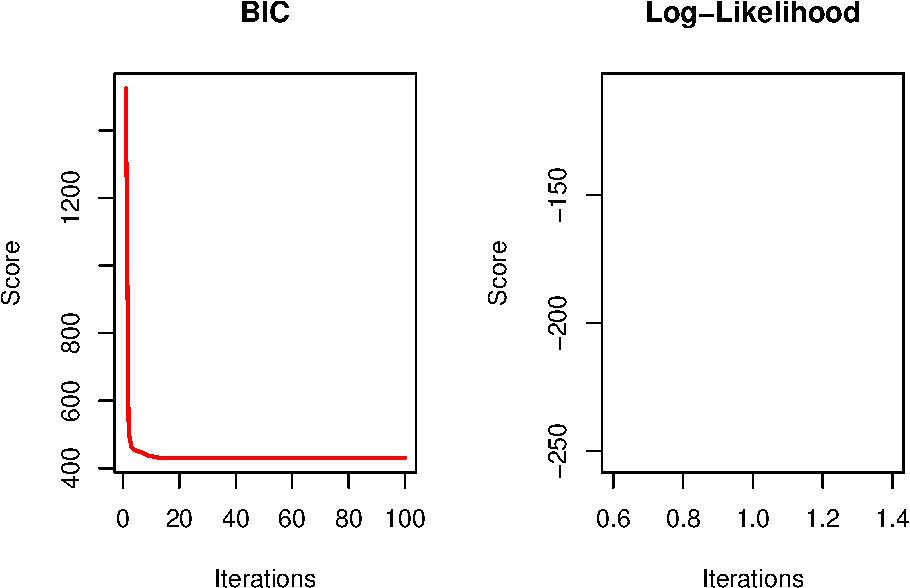
\includegraphics{exposition_files/figure-latex/unnamed-chunk-7-1.pdf}

\begin{Shaded}
\begin{Highlighting}[]
\CommentTok{\# Load the package}
\FunctionTok{library}\NormalTok{(mclust)}

\CommentTok{\# Select 4 continuous variables and look for three distinct groups.}
\NormalTok{mcl.model }\OtherTok{\textless{}{-}} \FunctionTok{Mclust}\NormalTok{(iris[, }\DecValTok{1}\SpecialCharTok{:}\DecValTok{4}\NormalTok{], }\DecValTok{3}\NormalTok{)}

\CommentTok{\# Plot our results.}
\FunctionTok{plot}\NormalTok{(mcl.model, }\AttributeTok{what =} \StringTok{"classification"}\NormalTok{, }\AttributeTok{main =} \StringTok{"Mclust Classification"}\NormalTok{)}
\end{Highlighting}
\end{Shaded}

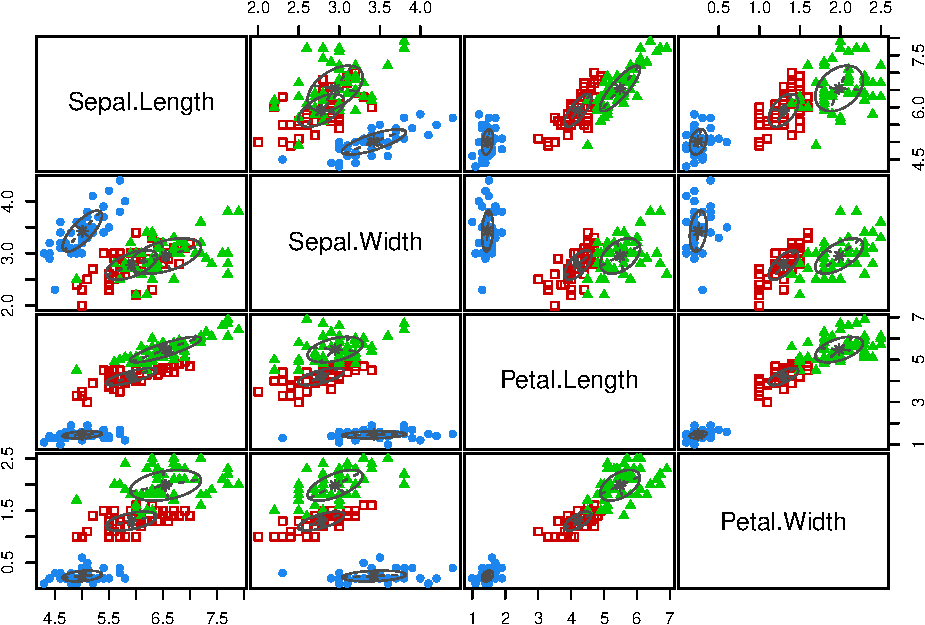
\includegraphics{exposition_files/figure-latex/unnamed-chunk-7-2.pdf}

\bibliographystyle{plainnat}
\renewcommand\refname{Conclusion}
\bibliography{bibliography.bib}



\end{document}
